% !TEX root = ../../thesis.tex

\chapter{Sensitivity of Building Properties and Use Types for the Application of Adaptive Photovoltaic Shading Systems}
\chaptermark{Sensitivity of Building Properties and Use Types}
\label{ch:asfArchetype}

\graphicspath{{chapters/ch3Archetype//Images/}}

\begin{chapterabstract}
AAn adaptive solar facade can improve building energy performance by controlling solar heat gains and natural lighting, while simultaneously generating electricity on site. The adaptive control of the solar facade is determined through an optimisation algorithm that minimises the net energy demand. In this paper, we first evaluate the sensitivity of the adaptive solar facade to the thermal performance of the building envelope for a south facing room in Zurich. We then evaluate the performance of an adaptive solar facade on 11 building use types spanning six construction periods. In addition, we compare the performance of an adaptive system against an equivalent static photovoltaic system, and a facade with no shading system. Our results show that the adaptive solar facade performs best in buildings that have a high cooling demand and low heating demand. This is because the optimum configurations for cooling minimisation generate the maximum photovoltaic electricity. As a result, we notice a higher energy saving potential in newer buildings with low envelope thermal transmittance (U-value or infiltration). However, in buildings with a very high cooling demand, and no heating demand, there is only a small improvement in performance compared to an equivalent static system. An adaptive solar facade is therefore an optimum solution when there are both heating demands, and cooling demands present. Modern offices, retail stores, food stores, and schools have this property and perform well with an adaptive solar facade compared to an equivalent static system, and a facade with no shading.
\end{chapterabstract}

\blfootnote{Jayathissa, P., Zarb, J., Hofer, J. \& Schlueter, A. Sensitivity of Building Properties and Use Types for the Application of Adaptive Photovoltaic Shading Systems. Energy Procedia, Proceedings to CISBAT (2017)}

\newpage

\section{Introduction}
\label{ch:introduction3}
% !TEX root = main.tex

Buildings are at the heart of society and currently account for 32\% of global final energy consumption and 19\% of energy related greenhouse gas emissions \cite{IPCC}. Nevertheless the building sector has a 50-90\% emission reduction potential using existing technologies, and widespread implementation could see energy use in buildings stabilise or even fall by 2050 \cite{IPCC}. Within this strategy, building integrated photovoltaics (BIPV) has the potential of providing a substantial segment of a building's energy needs \cite{defaix2012technical}. Even the photovoltaic (PV) industry has identified BIPV as one of the four key factors for the future success of PV \cite{raugei2009life}. \\

Recent developments regarding efficiency and costs of thin film BIPV technologies, in particular, CIGS, have brought new design possibilities \cite{NREL, kushiya2014cis, kaelin2004low, jelle2012building}. Their lightweight nature and customisable shapes allow for easier and more aesthetically pleasing integration into the building envelope. In addition, less power is required to actuate them, thus facilitating the development of dynamic envelope elements due to their reduced weight \cite{rossi2012adaptive}. \\





Dynamic buildings envelopes have gained interest in recent years because they can save energy by controlling direct and indirect radiation into the building, while still responding to the desires of the user \cite{loonen2013climate}. This mediation of solar insolation can offer a reduction in heating / cooling loads and an improvement of daylight distribution as seen in Figure \ref{fig:ASFschematic4} \cite{rossi2012adaptive}. Interestingly the structure and mechanics required for dynamic envelopes couples seamlessly with the structure and mechanics required for facade integrated PV solar tracking. The use of light weight PV as an adaptive envelope material enables it to also benefit from on-site energy production. Furthermore, it provides a new way of aesthetically integrating PV panels onto buildings. As discussed in Chapter \ref{ch:asfSimulation}, the balance of electricity production and adaptive shading can in some cases offset the entire energy demand of an office space behind the envelope \cite{jayathissa2015abs}. We have proposed one possible combination of these technologies as an Adaptive Solar Facade (ASF) \cite{nagy2016adaptive}. An example of an ASF can be seen in Figure \ref{fig:HoNR4}.




\begin{figure}
\begin{center}
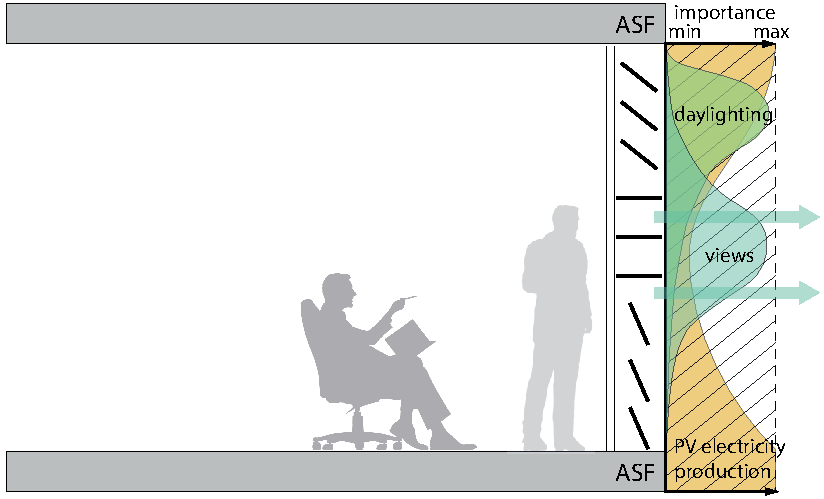
\includegraphics[width=8cm, trim= 0cm 0cm 0cm 0cm,clip]{facadeFunctions.pdf}
\caption{The facade acting as a mediator between the interior and exterior environment, while fullfilling various functions \cite{nagy2016adaptive}}
\label{fig:ASFschematic4}
\end{center}
\end{figure}

\begin{figure}
\begin{center}
\includegraphics[width=8cm, trim= 0cm 0cm 0cm 0cm,clip]{honr.jpg}
\caption{An example of an ASF constructed at the House of Natural Resources \cite{nagy2016adaptive}}
\label{fig:HoNR4}
\end{center}
\end{figure}

The design of an ASF comes at an added cost. The additional electronics, actuators, and supporting structure adds further embodied CO$_2$ to the product. It is therefore important to conduct a life cycle impact assessment (LCA) to analyse whether the life cycle environmental impacts are favorable, compared to a more classic system. It is also important to see how variations in design can alter the green house gas (GHG) reduction potential of the technology. Aspects such as the chosen actuator, control system, and location of operation can have an impact on environmental performance. 

The state of the art literature assesses existing photovoltaic technologies \cite{raugei2007life, de2013energy, fthenakis2011photovoltaics}, and the balance of systems (BOS) which includes all other components of a photovoltaic system \cite{mason2006energy}. This has not however, been expanded to dynamic BIPV systems, and in particular, systems that combine the benefits of adaptive shading and electricity production.\\


In this chapter, we investigate the environmental performance of an ASF and compare it to existing static photovoltaic systems. We also investigate 1) a system expansion including the heating ventilation and air conditioning (HVAC) savings through adaptive shading 2) design variations of the ASF, 3) the operational emissions of a building, with and without an ASF, and 4) the sensitivity of the LCA to its location and design.



The remainder of the chapter is organized as follows. The following section introduces the ASF and the used LCA methodology. In Section \ref{ch:results4}, we present the results of the LCA analysis. Section \ref{ch:discussion4} discusses the results and provides design guidelines. Section \ref{ch:conclusion4} concludes the chapter.



\section{Methodology}
\label{ch:method3}
% !TEX root = 99_main.tex

The parametric design environment (PDE), shown schematically in Figure \ref{fig:performative} details the multiple processes that were used in parallel to handle the different technological branches. From this, four key outputs are generated: the structural performance, energetic performance, manufacturing plans, and visual renders. Inputs to the PDE are defined by the parameters that have the greatest influence on the design. In this case, they are the overall frame dimension and profile, the photovoltaic panel dimension, spacing and layout, and the range of motion. 

These inputs are numerically fed into the design environment and generate instantaneous results of the structural performance, energetic performance, visual renders and manufacturing plans. By doing so, the multiple trade-offs between the technological branches, as explained in Section \ref{ch:introduction1}, can be simultaneously observed. The electricity generation, building energy demand, utilisation factor of yield strength, dimensions, collision detection, aesthetics, and manufacturing costs are of particular interest. This ultimately allows for quick feedback loops with the major stakeholders (architects, structural engineering, energy engineers, and production team) involved in the project. \\


The environment combines the geometric modelling software Rhinoceros 3D \cite{Rhino}, its parametric plug-in Grasshopper \cite{grasshopper}, and python \cite{python} as a scripting language. The relatively unspecialised nature of Rhino is complemented by a large number of specialised add-ons for Grasshopper. Furthermore, custom Grasshopper modules can be scripted using python. The following subsections will explain the structural and energetic analysis in more detail.

\begin{figure}
\begin{center}
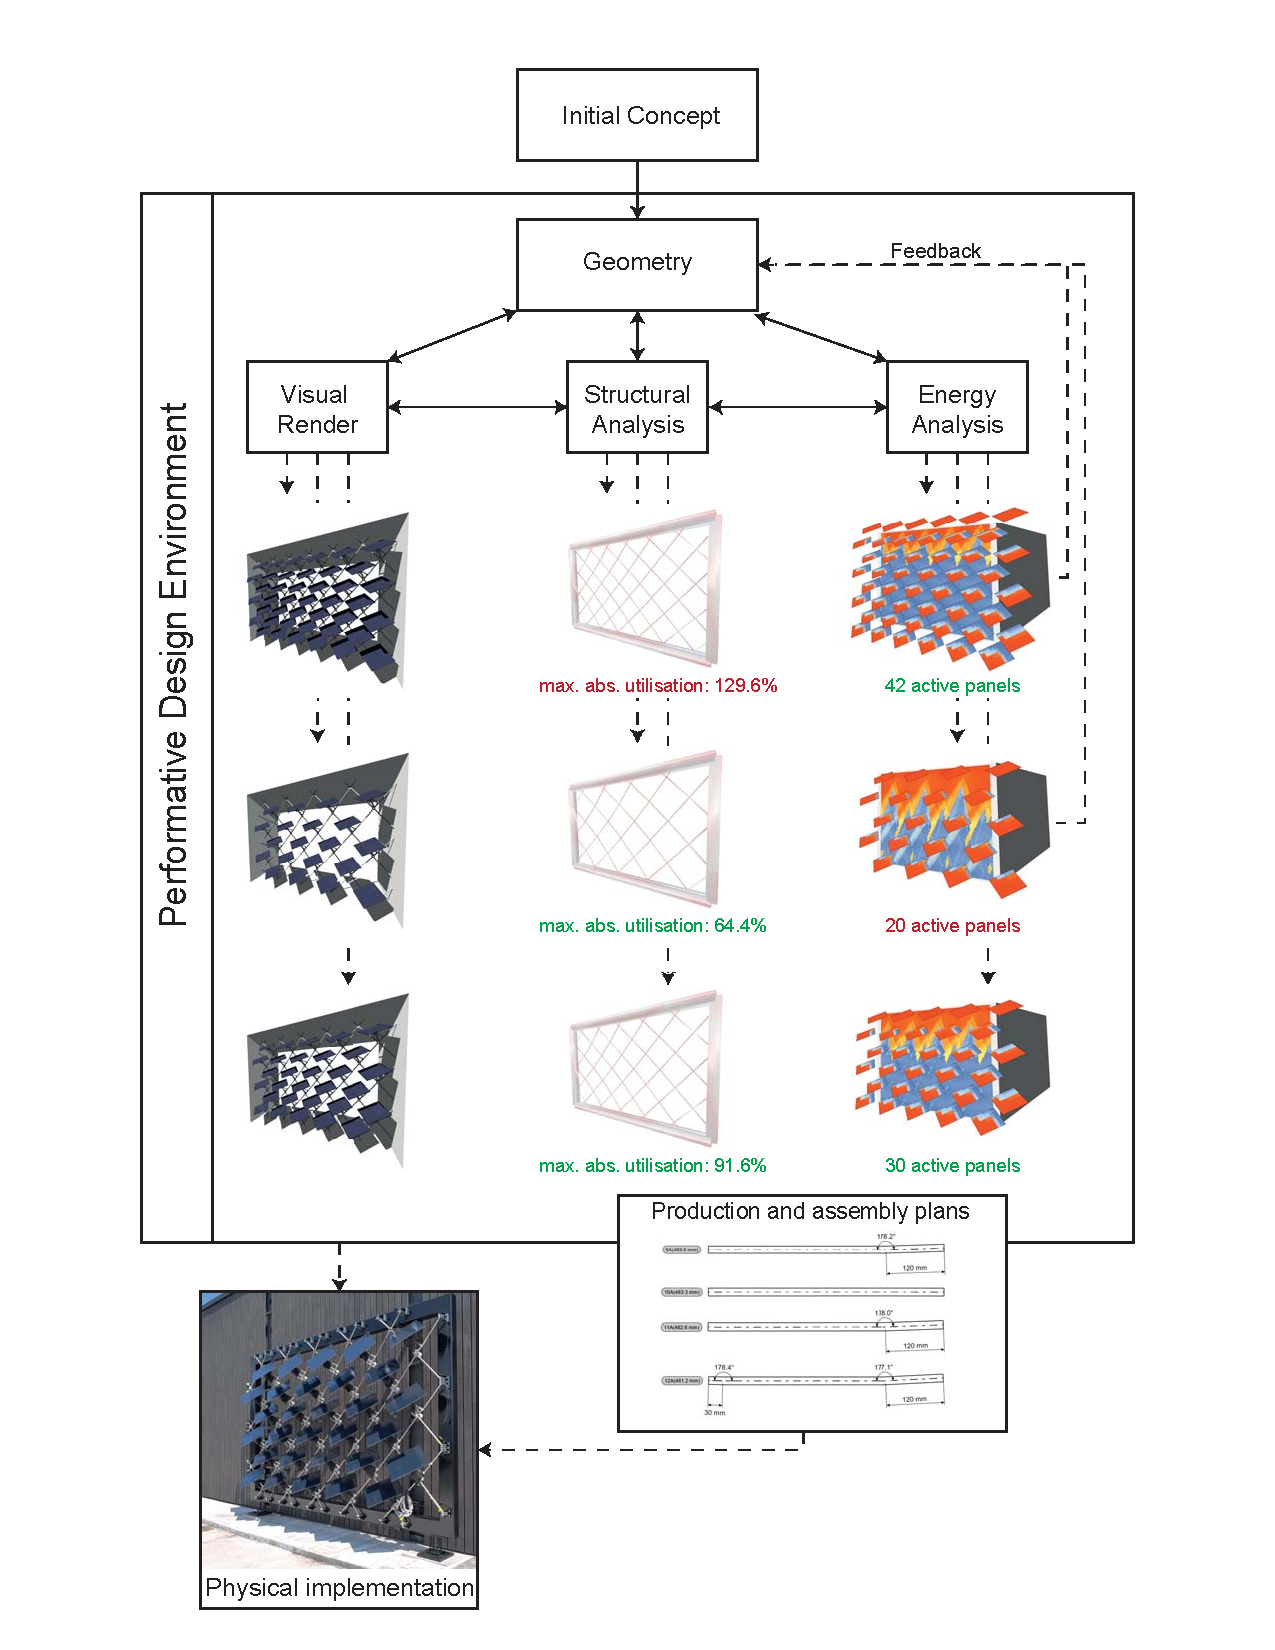
\includegraphics[width=\columnwidth, trim= 0cm 0cm 0cm 0cm,clip]{ASF_PDE_InfoGraphic.pdf}
\caption{The performative design environment is able to link four analysis methodologies for rapid design itterations}
\label{fig:performative}
\end{center}
\end{figure}

\subsection{Energy Evaluation}
\label{ch:energy}

The purpose of the ASF is to maximise electricity production on the photovoltaic (PV) panels and minimise the energy consumption of the building behind the facade. In order to best achieve this, the layout of the PV panels, and the electrical interconneciton of PV panels must be carefully designed.

The evaluation of the energetic performance of the ASF can be found in Chapter \ref{ch:asfSimulation}, and will be briefly reviewed here for completion. This part of the PDE consists of five stages: 

\begin{enumerate}
\item \textbf{Solar Radiation Model:} The radiation on the PV panels and window behind the ASF is calculated using the Grasshopper - LadyBug plugin.  \cite{roudsari2013ladybug}. An example of the simulation result is shown in Figure \ref{fig:radiation}. A tighter layout of panels allows for more PV material per facade area, however it also results in more module self-shading, which reduces the overall electricity production.
\item \textbf{PV Electricity Production:} The radiation result on the PV panels is coupled to an electrical circuit simulation of monolithically interconnected, thin-film CIGS PV modules. This model takes into account the effects of module self-shading and temperature dependence \cite{hofer2016parametric}. 
\item \textbf{Building Energy Model:} The radiation calculated on the window surface is fed to a 5R1C single zone resistance-capacitance building model based on the ISO 13790 standard \cite{de2008iso}. This calculates the heating or cooling demand of the building. A tight layout of PV panels enables more control over the solar insolation. Tight configurations tend to perform better in hot climates, whereas sparse configurations perform better in colder climates. 
\item \textbf{Daylighting Model:} A linear daylighting model based on the total flux methodology is used to determine the luminosity in the room \cite{szokolay1980handbook}. When the luminosity falls below a threshold value of 300lx, artificial lighting is turned on. Sparse configurations result in more daylight distribution, which reduces the need for artificial lighting in the morning and evening hours.
\item \textbf{Optimisation:} The simulation is conducted for all possible panel angle combinations for every hour of the year. By summing all the time steps, the annual energetic performance of the ASF can be evaluated. 
\end{enumerate}
This analysis finds the optimum balance between PV generation and daylight control to minimise heating, cooling and lighting demands where the overall objective is the minimisation of net energy.
The source code for this methodology, with installation instructions can be downloaded from github \cite{ASFGitHub,RCGitHub}.

During the design stage, this analysis is conducted for a typical day in summer, and in winter. Once a design has been selected, an annual study with hourly time steps is conducted to achieve a high resolution result.


\begin{figure}
\begin{center}
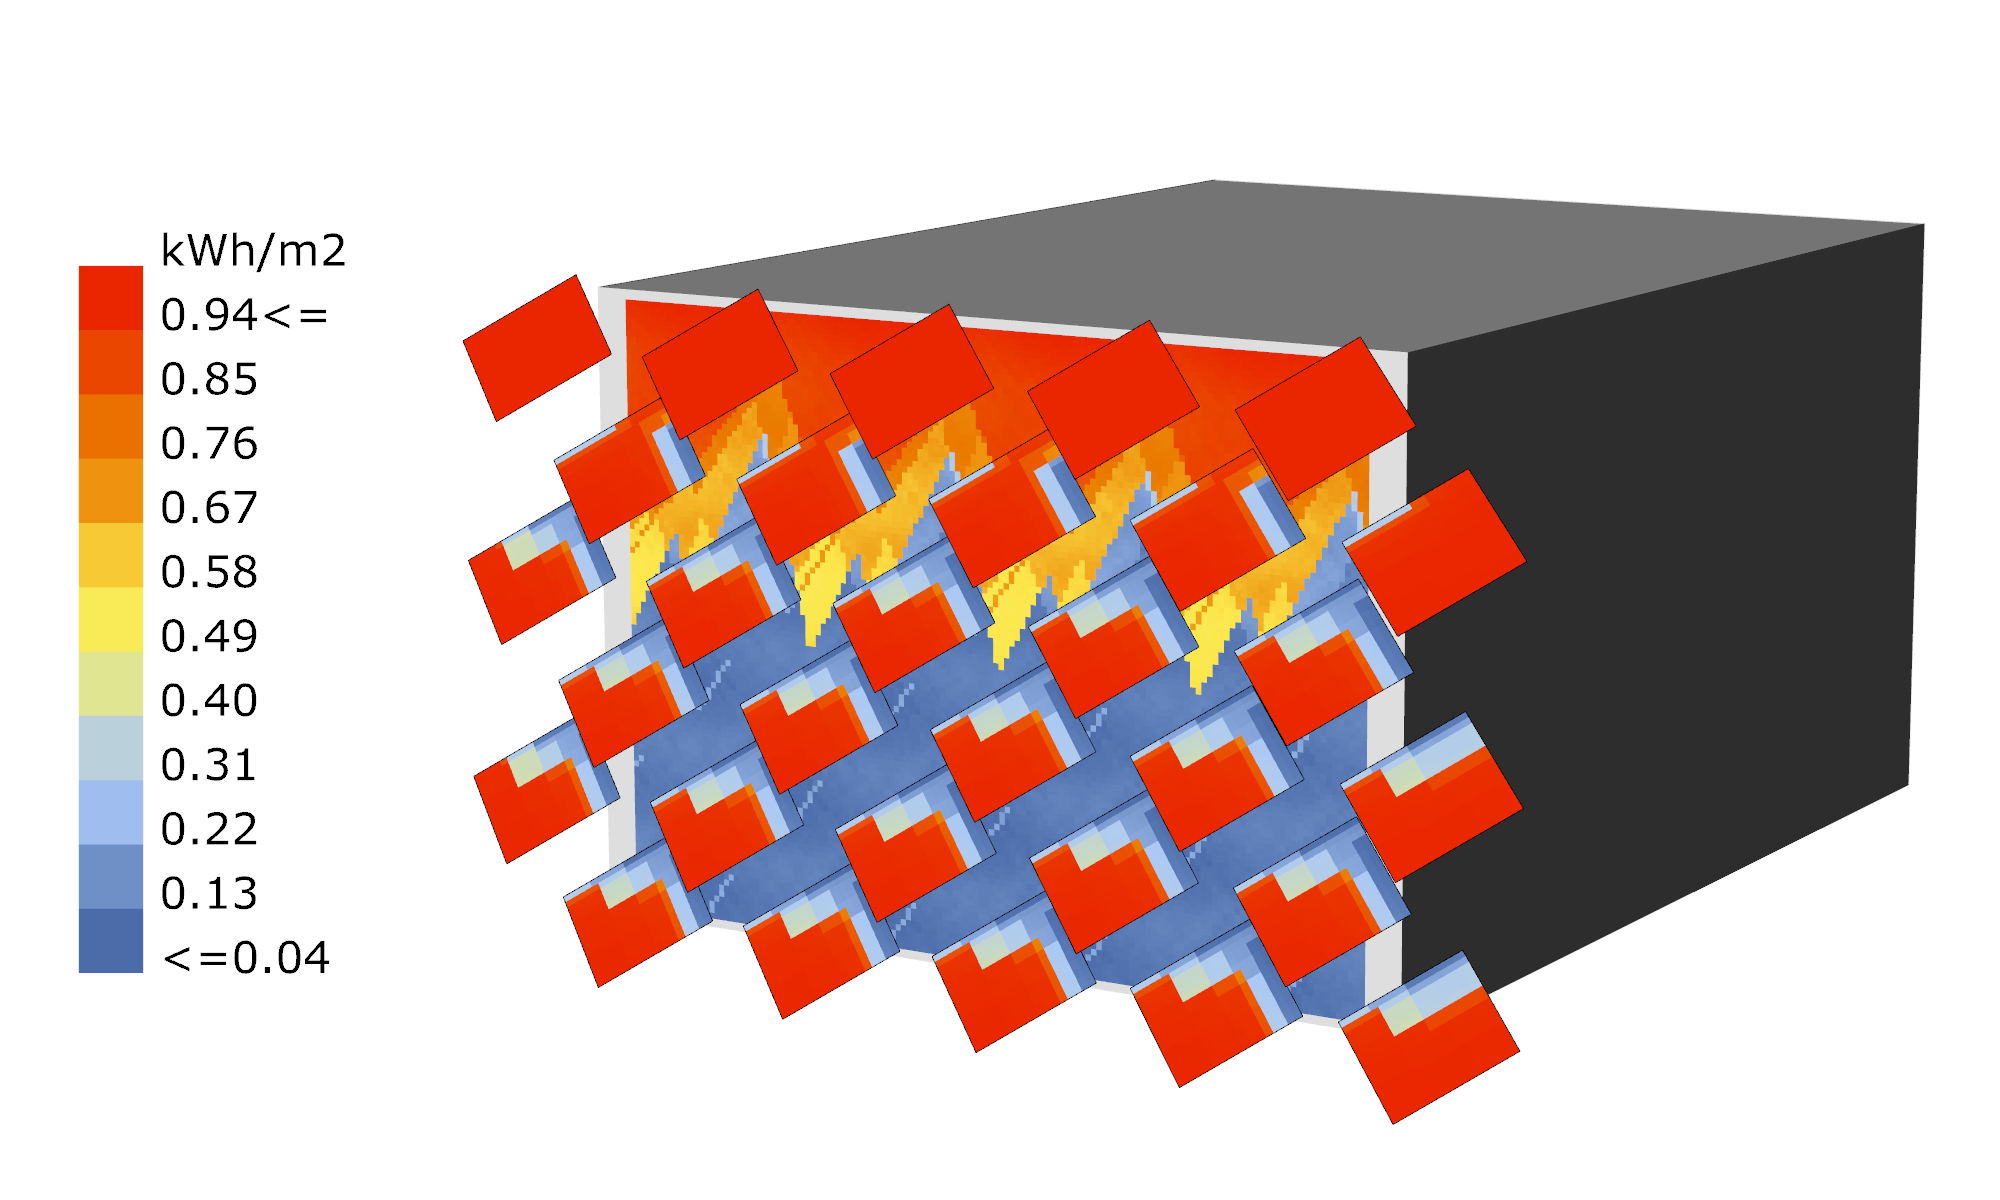
\includegraphics[width=\columnwidth, trim= 0cm 0cm 0cm 0cm,clip]{radiationHiLo2.png}
\caption{A simulation result showing the radiation on the solar panels and the window element on the 16 June 2013 between 12:00-13:00 in Zurich.}
\label{fig:radiation}
\end{center}
\end{figure}


\subsection{Structural form finding and finite element analysis}

The panel spacing, as discussed in Section \ref{ch:energy} can also influence the structural performance of the system, which in turn, influences the architectural image. It is therefore important to run the structural analysis in parallel to find the optimum solution. This subsection will first introduce the structural concept, and then detail how this concept was developed with the PDE.\\

The proposed ASF is based on a vaulted cross-hatched network of stainless steel pipes as seen in Figure \ref{fig:structure}. The junctions where the pipes cross serve as the mounting points for each dynamic photovoltaic module. All utility lines are routed within the pipe network. A steel frame supports the pipe network to create a stand-alone pre fabricated component, which can be mounted directly to the building envelope. The vaulted shape further strengthens the structure against wind loads, thus allowing for thinner pipe diameters, which increases transparency. \\


The form of the vaulted structure is determined through RhinoVault, a form finding plug in for Grasshopper \cite{Rippmann2012}. The method calculates the optimum shape of the pipe network based on the loading points and inputs to the design environment. Once the form is determined, a structural second order finite element analysis is conducted using the Karamba3d plug-in \cite{karamba} to dimension the structural elements. Further manual adjustments to the mesh can be conducted to improve the architectural image. Each manual adjustment is directly computed by the second order FEA module, providing real time feedback about the stability of the adjusted structure.  Figure \ref{fig:structureSettings} shows an example of this output with a list of simulation parameters. A load of 420N was applied on each panel node, which is equivalent to a category one hurricane on the Saffir-Simpson scale. The results are visualised in the form of coloured meshes which detail the utilisation factor in relation to the von Mises stress. A scaled down 2.2m x 1.5m prototype was constructed to validate the structural model. 

\begin{figure}
\begin{center}
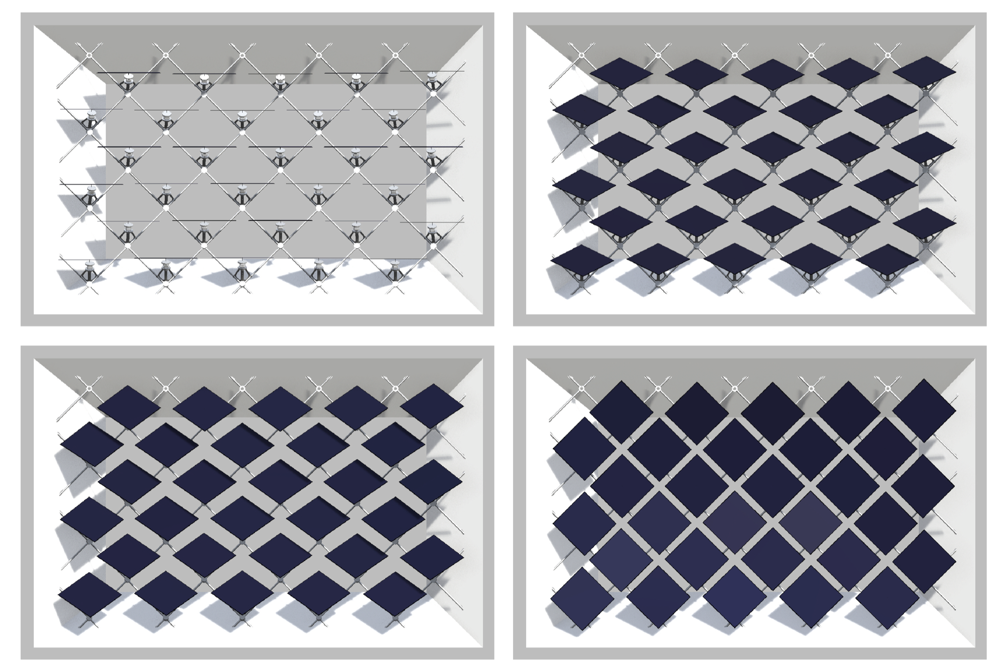
\includegraphics[width=\columnwidth, trim= 0cm 0cm 0cm 0cm,clip]{HiLoFrontRenderSmall.png}
\caption{The Adaptive Solar Facade existing in varying states}
\label{fig:structure}
\end{center}
\end{figure}

\begin{figure}
\begin{center}
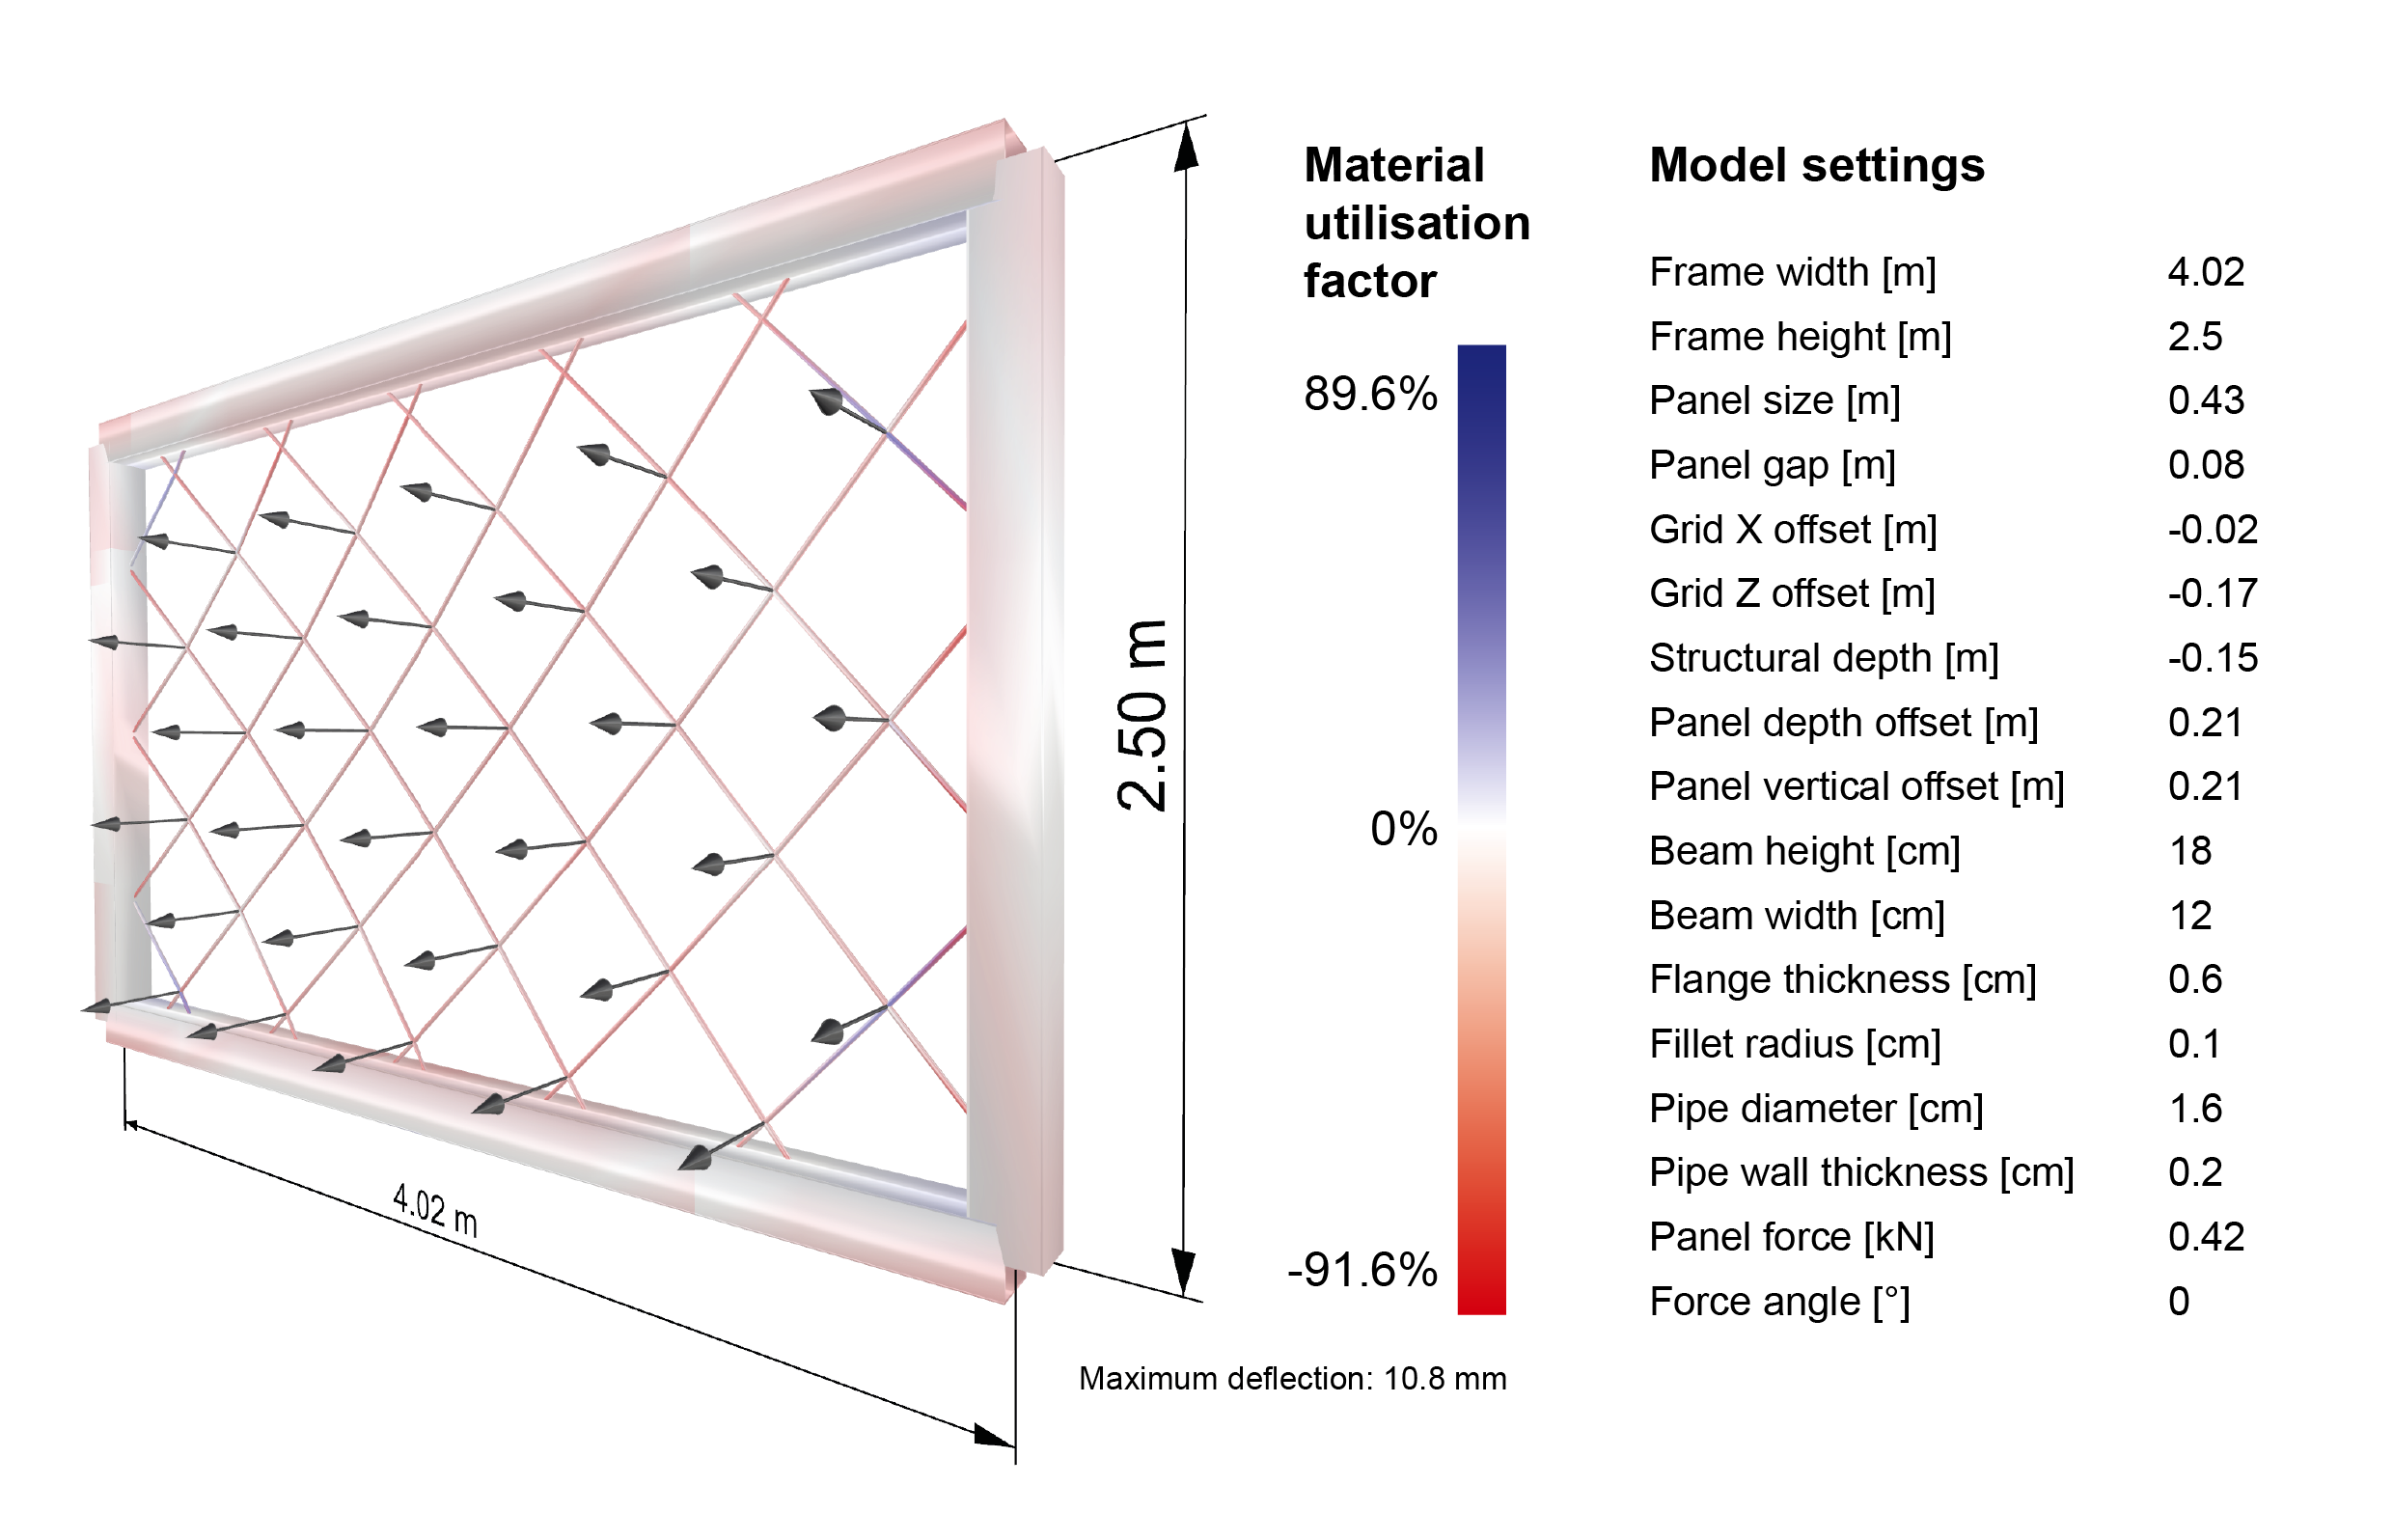
\includegraphics[width=\columnwidth, trim= 0cm 0cm 0cm 0cm,clip]{HiLo_ASF_Structural_Simulation.png}
\caption{An example output from the Karamba structural simulation. The black arrows detail the loading direction, and the colour details the utilisation factor in relation to the von Mises stress. The table on the right details the input parameters to the simulation.}
\label{fig:structureSettings}
\end{center}
\end{figure}




\subsection{Integration of classical design methods}

A purely parametric approach is very useful in investigating design possibilities, but once the concept needs to be put in practice, the parametric design environment needs to be complemented with physical prototypes, testing and classical design methods like simple 3D modelling and electronics design.
As there is a trade-off  between the  flexibility of a parametrised environment and the time required for its development, it is important to wisely choose what to parametrise and what to design with classical methods. Parametrising the entire design process of complex systems such as an ASF can result in instabilities and lead to an increase in design time. For this reason, it is important to include certain constants amongst the parametric variables. Constants include the design of the electronics, connection details, and the actuator design \cite{Svetozarevic2017a,svetozarevic2016soro}.




\section{Results}
\label{ch:results3}
% !TEX root = 99_main.tex

\subsection{Sensitivity of the Building Envelope}
\label{ch:envelope}

Figure \ref{fig:envelopeASF} details the performance of the ASF constructed on a typical office building with respect to the envelope U-value. As expected the heating demand increases with increasing U-value. Interestingly, the photovoltaic electricity supply decreases. This is because the ASF always optimises for net energy minimisation. With increasing heating demands, the ASF will optimise for positions that direct solar radiation into the building to minimise the heating loads as opposed to generating the electricity on the panels. This same characteristic is apparent in \ref{fig:envelopecompNo} which compares the energy saving potential of the ASF compared to a glazed facade with no shading system. A building with low envelope U-value will have a large saving potential due to the reduction of cooling loads, and supply of photovoltaic electricity. As the envelope U-value increases, this saving potential begins to decrease.

Figure \ref{fig:envelopecompstatic} compares the ASF to an equivalent static photovoltaic shading system with panels orientated in the most energetically favourable position. As the U-value increases the net energy saving increases. As mentioned earlier, the heating demand increases with increasing U-value. For high U-value envelopes, the ASF will adapt and open up the panels thus reducing the heating demands. The equivalent static system will remain in a semi closed position for the entire year, and will block the solar heat gains necessary in winter.

Figure \ref{fig:infiltration} details the equivalent analysis with varying infiltration rates. Similar trends can be observed to those in Figure \ref{fig:envelope}. Leakier buildings lead to high heat demands, which decreases the performance of the ASF compared to a glazed window with no shading, but increases the performance relative to a static shading system. 



\begin{figure}
    \centering
    \begin{subfigure}[b]{0.47\textwidth}
        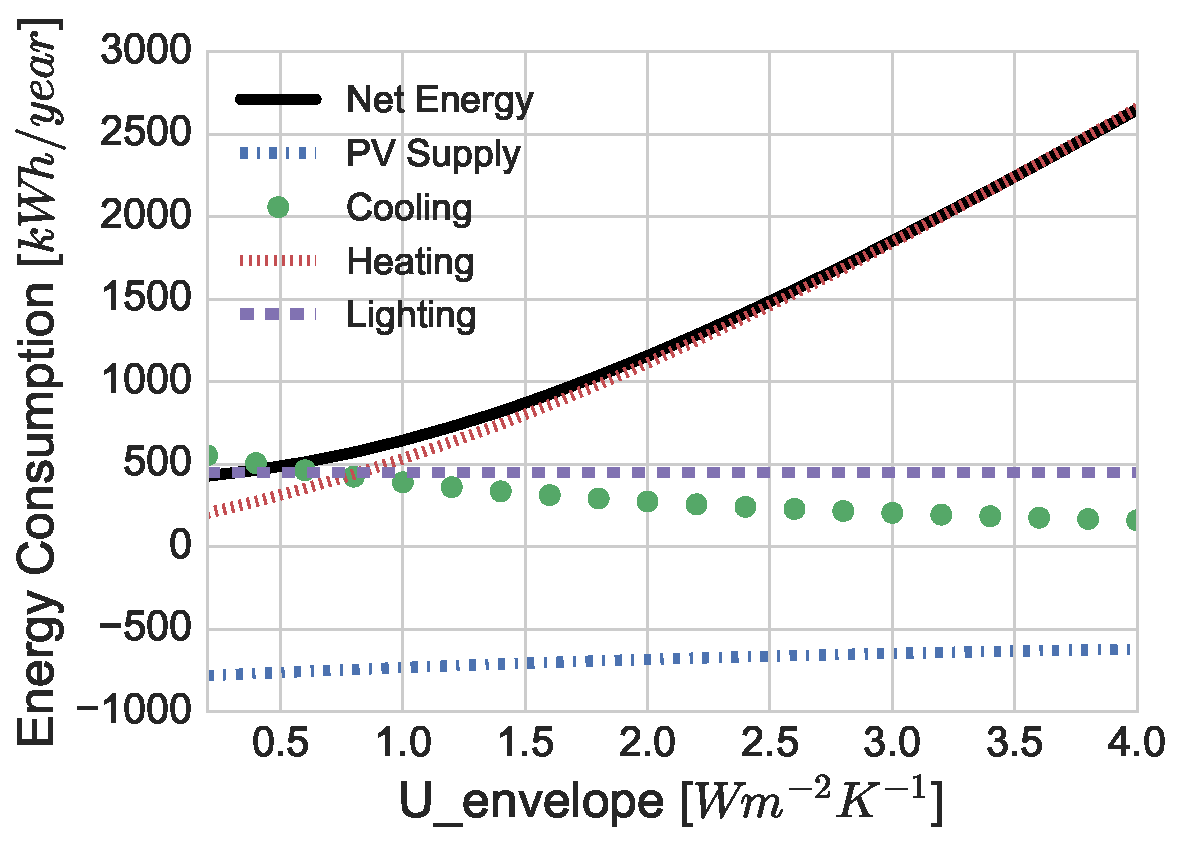
\includegraphics[width=\textwidth]{Sensitivity_ZH_U_env_COP3_1_ASF.pdf}
        \caption{} 
        \label{fig:envelopeASF} 
    \end{subfigure} \vfill
    \begin{subfigure}[b]{0.47\textwidth}
        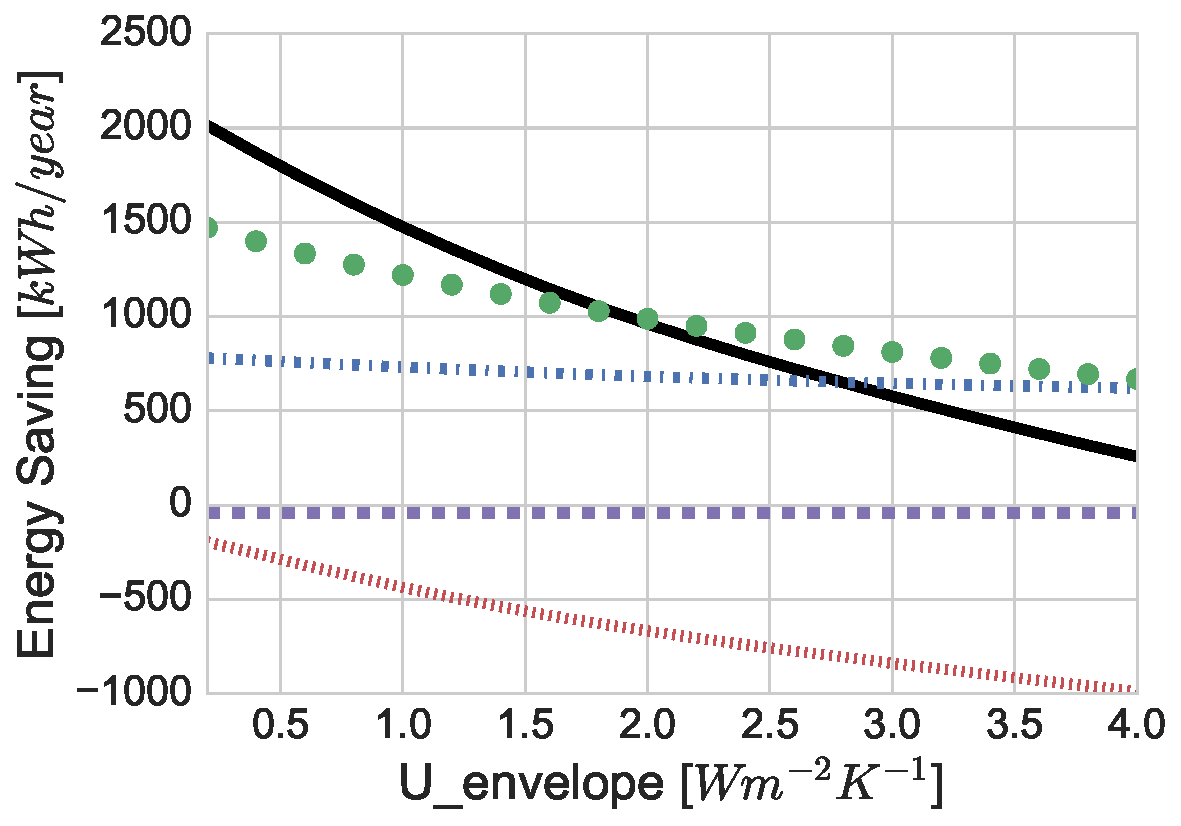
\includegraphics[width=\textwidth]{Sensitivity_ZH_U_env_COP3_1EnergySavingNoASF.pdf}
        \caption{}
        \label{fig:envelopecompNo} 
    \end{subfigure} \hfill
    \begin{subfigure}[b]{0.47\textwidth}
        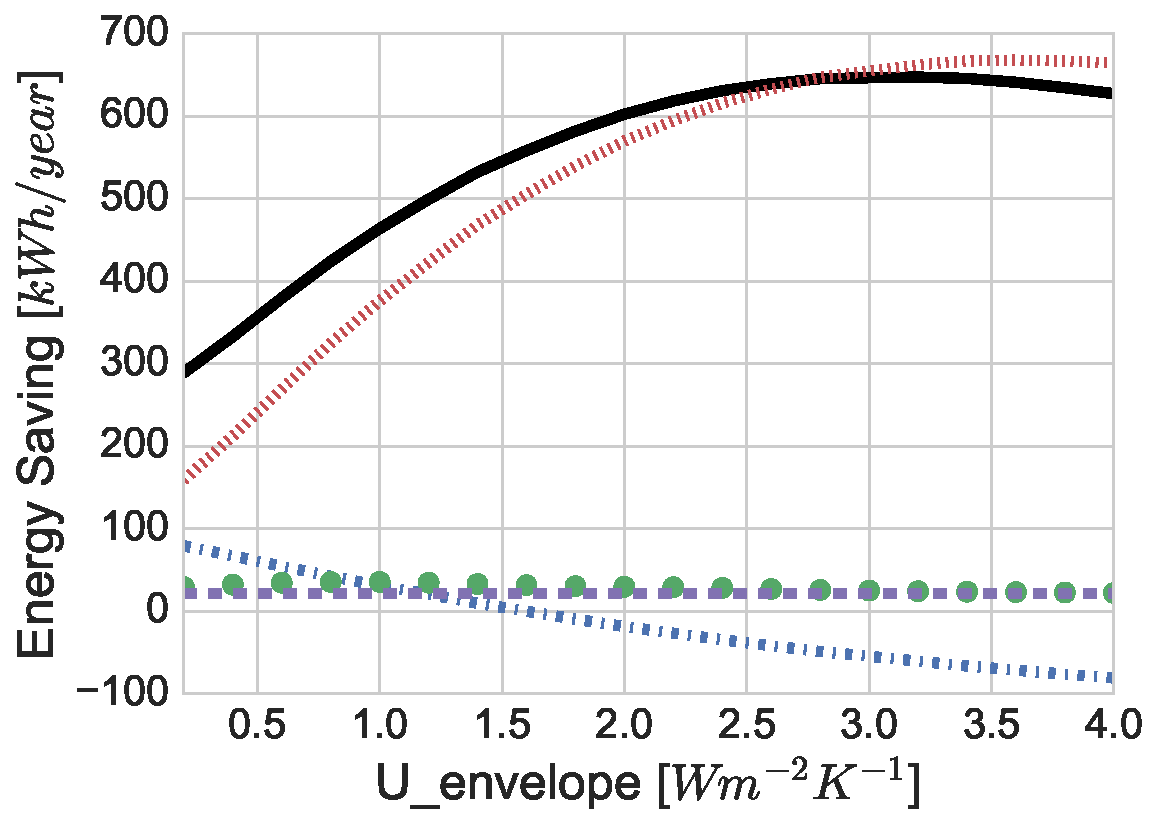
\includegraphics[width=\textwidth]{Sensitivity_ZH_U_env_COP3_1EnergySavingStatic.pdf}
        \caption{}
        \label{fig:envelopecompstatic} 
    \end{subfigure} 
    
    \caption{Influence of envelope thermal transmittance (U-value). a) Details the energetic performance of the ASF with respect to building envelope U-value. b) compares the energy saving potential of an ASF relative to a facade with no shading system. c) compares the energy saving potential of an ASF relative to an equivalent static PV system. }
    \label{fig:envelope}
\end{figure}


\begin{figure}
    \centering
    \begin{subfigure}[b]{0.47\textwidth}
        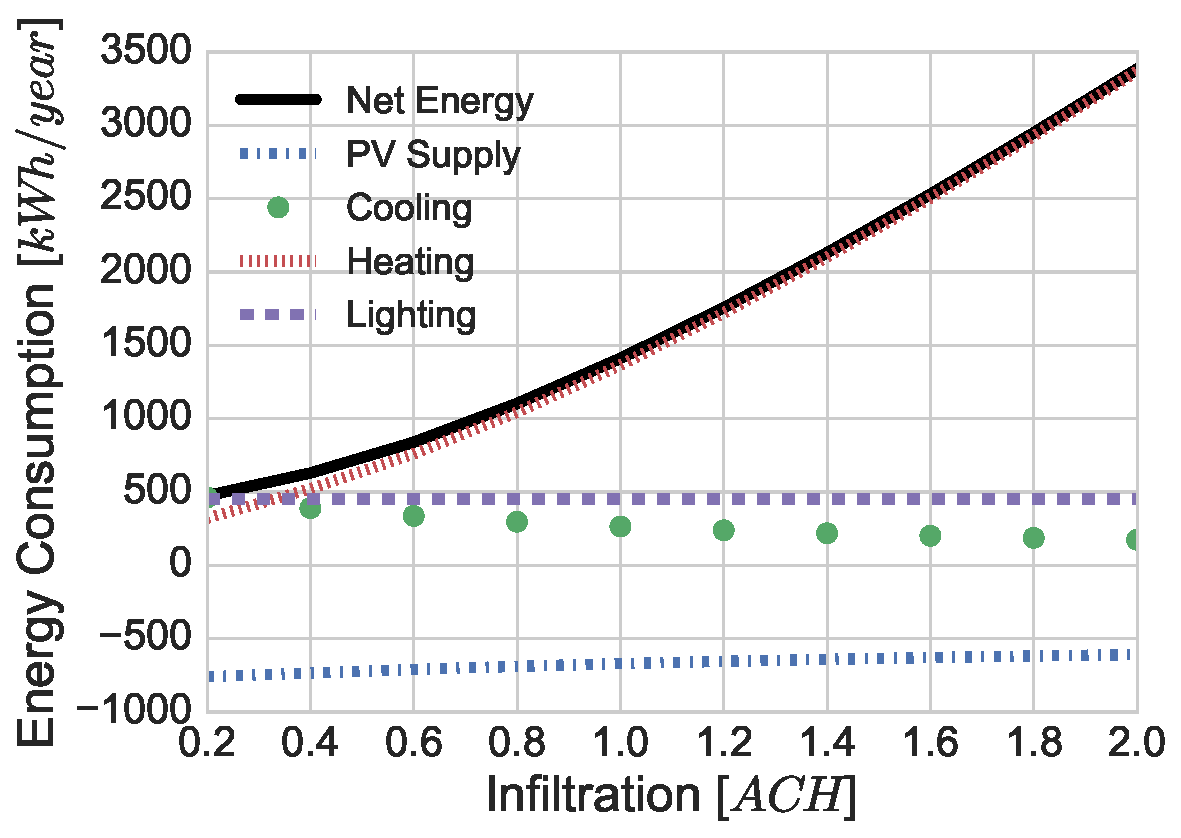
\includegraphics[width=\textwidth]{Sensitivity_ZH_Infl_COP3_1_ASF.pdf}
        \caption{} 
        \label{fig:infiltrationASF}
    \end{subfigure} \vfill
    \begin{subfigure}[b]{0.47\textwidth}
        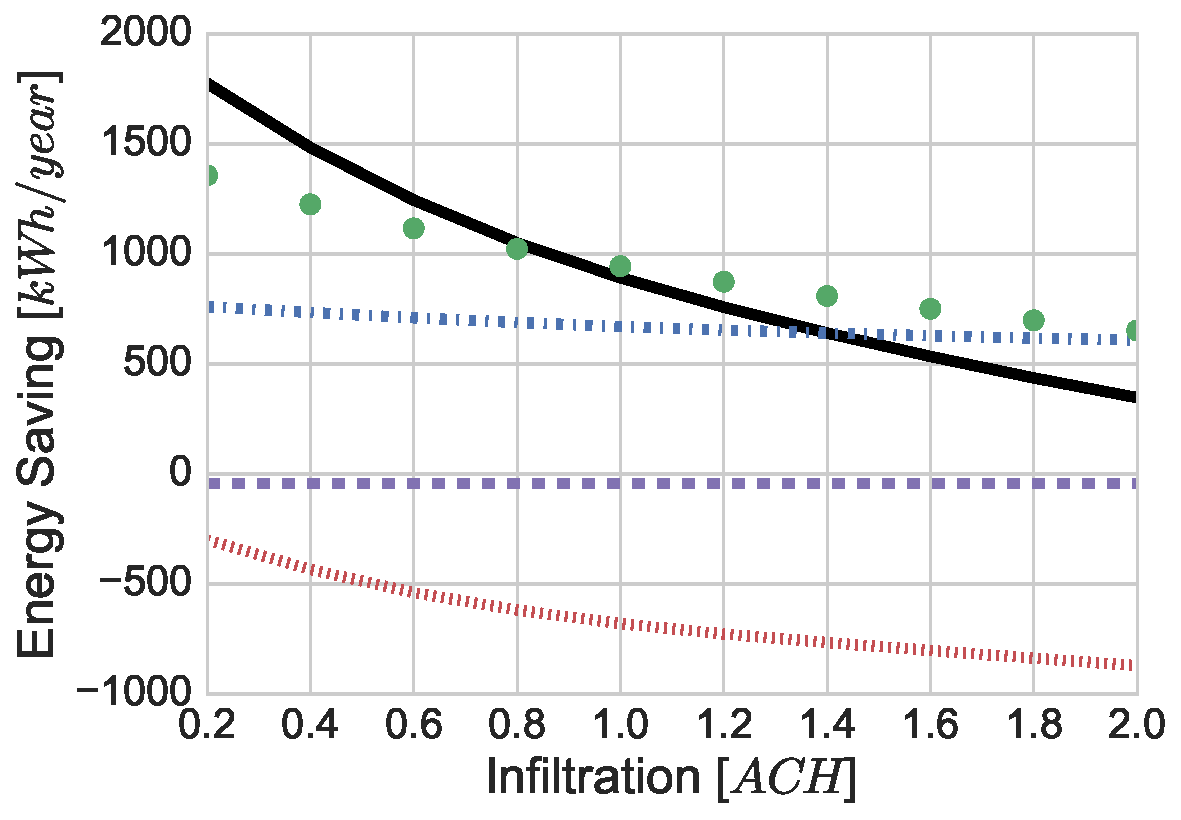
\includegraphics[width=\textwidth]{Sensitivity_ZH_Infl_COP3_1EnergySavingNoASF.pdf}
        \caption{}
        \label{fig:infiltrationcompNo}
    \end{subfigure}\hfill
    \begin{subfigure}[b]{0.47\textwidth}
        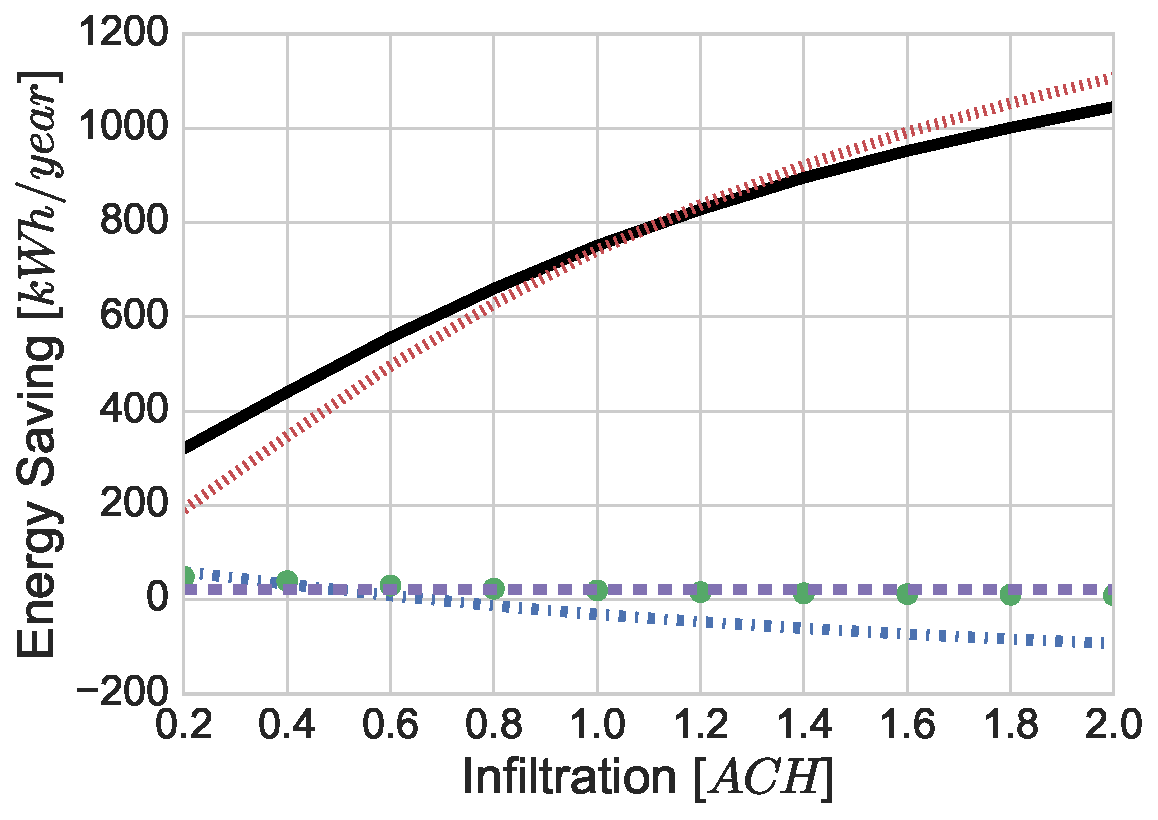
\includegraphics[width=\textwidth]{Sensitivity_ZH_Infl_COP3_1EnergySavingStatic.pdf}
        \caption{}
        \label{fig:infiltrationcompstatic}
    \end{subfigure}
    \hfill
    \caption{Influence of infiltration. a) Details the energetic performance of the ASF with respect to building infiltration. b) compares the energy saving potential of an ASF relative to a facade with no shading system. c) compares the energy saving potential of an ASF relative to an equivalent static PV system.}
    \label{fig:infiltration}
\end{figure}


\subsection{Archetype Evaluation of the ASF}

Figure \ref{fig:ArchResultsNoASF} compares the energy saving potential of 11 building use types with six different construction periods compared to a glazed facade with no shading system. Darker colours indicate larger energy saving potentials. One clear trend is the increasing saving potential in newer buildings over older buildings. This can be attributed to the lower envelope U-value in newer buildings, which as discussed in Section \ref{ch:envelope} will increase the energy saving potential. It is also interesting to note that the ASF performs best in gym use types. Gyms have a large cooling demand due to the high human heat emissions. Optimum configurations for cooling minimisation generates the maximum photovoltaic electricity supply. 


However, an ASF is not necessarily the best design solution for buildings with a large cooling demand. Figure \ref{fig:ArchResultsStatic} compares the ASF performance against an equivalent static system. If we once again focus on the modern gym, we notice that there is only a small increase in the energy performance of an adaptive system over an optimally configured static system. When comparing both heat maps we see that an ASF performs best on in a modern office, retail store, food store, and school. These archetypes perform well due to two reasons. Firstly, they have an even balance of heating and cooling demands. Thus there is a need for adaptivity in the envelope to reduce these demands. Secondly, these archetypes are in use during the day. Residential buildings on the other hand are mostly occupied at night where the ASF has no influence on the building performance.

\begin{figure}
\begin{center}
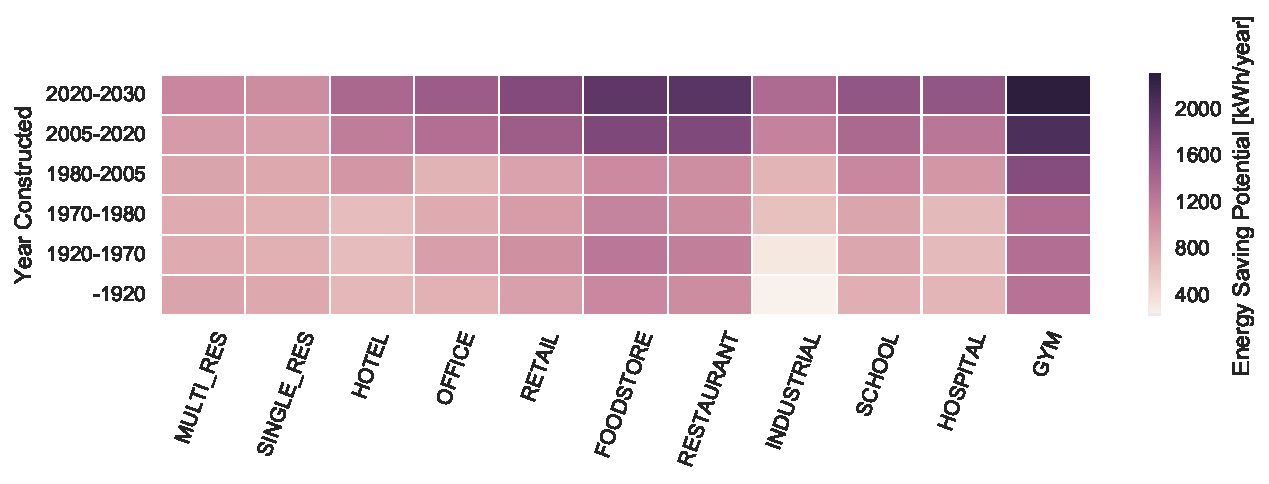
\includegraphics[width=\textwidth, trim= 0cm 0cm 0cm 0cm,clip]{energySaving_COP1_3_NoASF.pdf}
\caption{Annual results detailing the energy saving potential of the ASF vs a glazed window with no shading system}
\label{fig:ArchResultsNoASF}
\end{center}
\end{figure}

\begin{figure}
\begin{center}
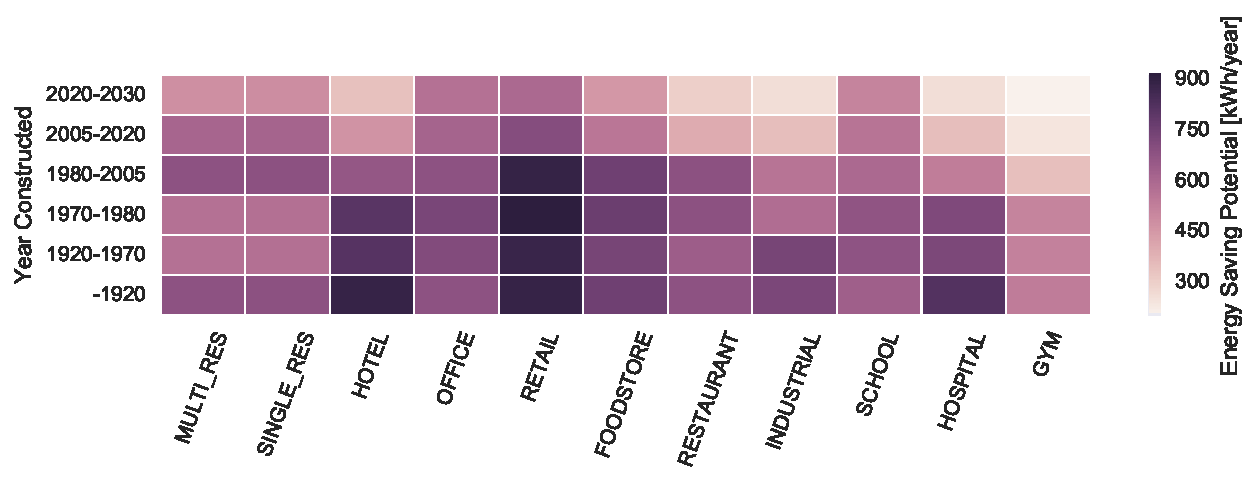
\includegraphics[width=\textwidth, trim= 0cm 0cm 0cm 0cm,clip]{energySaving_COP1_3_static.pdf}
\caption{Annual results detailing the energy saving potential of the ASF vs a static photovoltaic shading system}
\label{fig:ArchResultsStatic}
\end{center}
\end{figure}



% \section{Discussion}
% \label{ch:discussion}
% \input{5_discussion}

\section{Discussion and Conclusion}
\label{ch:conclusion3}
% !TEX root = 99_main.tex

This paper presents a practical PDE for the design and fabrication of kinetic architectural elements. The PDE is capable of combining the multiple fields of structural engineering, energy engineering, control engineering, industrial design and architecture into one uniform environment, allowing the designers to handle the complexities of a multidisciplinary project. 

The major advantage of this environment is the considerable decrease in time between design iterations. Traditionally each of the respective stakeholders in the project would work on their individual design, and then exchange information in a meeting. With the PDE, the meeting is transformed from an information exchange session, to a design session where all stakeholders can collaboratively influence the design and immediately see the necessary results. What would normally take a month, was condensed to just a few hours. The design environment also develops with the project allowing for new parametric inputs, or new outputs to be created. This can be easily done with collaborative software management tools such as git.

One disadvantage is the overhead required to manage a PDE. Like a BIM manager, a PDE manager is required and must have a careful overview of the software. As the software ultimately determines the final form of the design, any errors in the software can be detrimental to the final design. It was therefore necessary for all stakeholders to conduct a final independent analysis prior to the submission of the final design. 

It is also important to determine what aspects of the design should be contained within the PDE and what should be designed with classical methods. Essentially, all aspects where there could be conflicts between the stakeholders were included in the PDE, whereas many of the design details, such as the mounting brackets to the building, can still be designed independently and imported into the PDE as a static object. Over time, some static objects, such as the cantilevered bracket of the PV module became parametrised. 

Ultimately, this paper presents a further step in the field of performative design by showing how a system as complex as a kinetic photovoltaic envelope, can be developed, prototyped and finally fabricated by a small team of four designers. The methodology can be utilised for any building component where multiple technological branches are required.




% \dictum[James C. Maxwell]{%
%   The true logic of this world is in the calculus of probabilities. }%
% \vskip 1em

% \Citet{Maxwell1865} derived some very useful equations for electromagnetic
% fields:
% \begin{align}
%     \nabla \cdot \vec{D} = \rho \\
%     \nabla \cdot \vec{B} = 0 \\
%     \nabla \times \vec{E} = -\frac{\partial \vec{B}}{\partial t} \\
%     \nabla \times \vec{H} = \vec{j} + \frac{\partial \vec{D}}{\partial t}
% \end{align}

% The energy--momentum relation, \cref{eq:energy-momentum}, is one of \emph{my}
% important results:
% \begin{align}
%     E^2 = m^2 c^4 + (p c)^2 \label{eq:energy-momentum}
% \end{align}

% Write units like this: \u{5}{\micro\meter}.

% \begin{figure}
%   \caption{A lovely face.}
% \label{fig:some-figure}
% 
\includegraphics{\dir/figure.pdf}
% \end{figure}
